\documentclass[11pt]{article}
\usepackage{amsmath,amsfonts}
\usepackage[numbers,sort&compress]{natbib}
\usepackage{times}
\usepackage[left=2.54cm,top=2.54cm,right=2.54cm,bottom=2.54cm,bindingoffset=0.0cm]{geometry}
\usepackage{setspace}
\usepackage{enumerate}
\usepackage{enumitem}
\usepackage{wrapfig}
\setcounter{secnumdepth}{0}
\usepackage{fullpage}
\usepackage{titlesec}
\titleformat{\section}{\large\bfseries}{\thesection}{1em}{}
\titleformat{\subsection}{\bfseries}{\thesubsection}{1em}{}
\usepackage{parskip} % skip paragraph indentations
\usepackage{lipsum}
\usepackage{hyperref}
\usepackage{graphicx}
\usepackage{amssymb}
\usepackage[x11names]{xcolor}
\usepackage{hyperref}
\usepackage{enumitem}
\usepackage{booktabs}
\usepackage{amsmath}
\usepackage{amssymb}
\usepackage{mathrsfs}
\usepackage{caption} \captionsetup[table]{singlelinecheck=false} %makes table captions left-justified
\usepackage{framed} % to add frames around comments
%\hypersetup{backref,colorlinks=false,
%    urlbordercolor=LightSkyBlue4,          % color of internal links
%    citebordercolor=SpringGreen4,        % color of links to bibliography
%    filebordercolor=magenta,      % color of file links
%    linkbordercolor=Red3, pdfborderstyle={/S/U/W 1.5}}
\newcommand{\Prob}[1]{\Pr{\left( #1 \right)}}
\newcommand{\q}[1]{``#1''} % easier way to get double quotes
\newcommand{\argmin}{\text{argmin}}
\usepackage{authblk} % for title page
\renewcommand\Affilfont{\fontsize{10}{10.8}\itshape}
\renewcommand\familydefault{\sfdefault} 
\usepackage{datetime2}
%\renewcommand{\dateseparator}{-}
\usepackage{atbegshi}% http://ctan.org/pkg/atbegshi -- removes blank page at start of doc
\AtBeginDocument{\AtBeginShipoutNext{\AtBeginShipoutDiscard}}
\setcounter{page}{0}

\lhead{Large groups and poor memory favor learning about badges}


\begin{document}
\noindent
\title{Large groups and poor memory favor learning about badges of status over individual recognition} 
\author{}
\date{} 
\maketitle

%Target journal: Behavioral Ecology 
%instructions: http://www.oxfordjournals.org/our_journals/beheco/for_authors/general.html
% also: http://www.oxfordjournals.org/our_journals/beheco/for_authors/submission_online.html

%%%%%%%%%%%%%%%%%%%%%%%%%%%%%%%%%%%%
\linenumbers

\section*{Lay summary}
Animals that live in groups need to have a way to learn about other members of their group. Some animals are able to recognize each individual in their groups. Others can only tell two animals apart if the signals they display are different enough. We find that learning is always more difficult in large groups and when animals have poor memory. In these cases, it is better to learn about categories of signals of others, rather than relying on learning about specific individuals.

%%%%%%%%%%%%%%%%%%%%%%%
\section*{Abstract}
%%%%%%%%%%%%%%%%%%%%%%%
Animals in social groups benefit from having accurate information about their group mates. Different species have different methods for gathering this information: some animals recognize members of their groups as individuals, while others coarsely categorize conspecifics based on observable traits. In many animals, a property of interest, for example dominance or health, is correlated with an otherwise unimportant trait, which is then referred to as a badge of status. Much is known about the circumstances that promote the evolution of either individual recognition or a badge of status, but there are few studies that compare the effectiveness of the two systems of learning. In order to study how group size and cognitive abilities influence the effectiveness of both types of learning and to determine the circumstances under which one is preferable, we develop and analyze a simple model of an animal social group, in which animals learn by interacting with each other and by observing these interactions. Regardless of how the animals assess the quality of their group mates, we find that larger group sizes and longer memory windows make it easier to learn more accurately and more quickly. We also find that intermediate perceptive abilities maximize the effectiveness of learning about a badge of status and that observational learning is more beneficial for animals using individual recognition. Finally, we find that learning about a badge of status is less costly than individual recognition when animals live in large groups, have short memories, and have coarse perceptive abilities.



\textbf{Keywords:} badge, cognition, evolution, learning, recognition, signal, social groups

\newpage
%%%%%%%%%%%%%%%%%%%%%%%
\section*{Introduction} 
%%%%%%%%%%%%%%%%%%%%%%%
Animals in social groups benefit from having accurate information about their group mates \citep{Seyfarth:2010bh}. Knowledge of the dominance ~\citep{Waal:1986ys,Cowlishaw:1990vn,Bergman:2003qf,Seyfarth:2005ve,Flack:2006uq,Hobson:2015uq}, resource holding potential~\citep{Rhijn:1980uq,Freeman:1985kl,Dick:1990cr,Lemel:1993ve}, likelihood of investing in parental care~\citep{Qvarnstrom:1997fk,Olsen:2010uq}, or health~\citep{Folstad:1992kx,Loyau:2005nx} of other animals can help an animal decide with whom to fight, mate, or interact. In order to learn about one's group mates, an animal must be able to differentiate among them. There are many solutions to this problem. Some animals recognize other members of their groups as individuals. Other animals coarsely categorize conspecifics based on traits they exhibit. In many animals, a property of interest, for example dominance or health, is correlated with an otherwise unimportant trait, which is then referred to as a badge of status~\citep{dawkins1978signals,Rohwer:1981vn,Rohwer:1982fk} and can allow animals to make inferences about each others' quality as mates or opponents or allies. 

Much is known about what circumstances might promote the evolution of one or the other type of learning (e.g. \citep{Whitfield:1987tg,Rohwer:1975fk,Lemel:1993ve,Solberg:1997uq,Tibbetts:2009kx,Remy:2010fk,Sheehan:2014fk}), but there are few studies that compare the two systems directly \citep{sheehan2016evotradeoff}. Our goal in this paper is to compare badge and individual recognition systems. In order to study how group size and cognitive abilities influence the effectiveness of both types of learning and to determine the circumstances under which one is preferable, we develop and analyze a simple model of an animal social group, in which animals learn by interacting with each other and by observing these interactions.  

% summary of previous research on badges
There are many species in which animals have been shown to use badges of status to make inferences about each other. One well known-example is the house sparrow: the size of a male sparrow's black bib is correlated with its physical condition and other sparrows seem to use this information to decide how to interact with a given male \citep{Moller:1987vn,Veiga:1993fk}. Another well-studied example is a species of paper wasp: the extent of black and the number of black patches on a wasp's face are positively correlated with its dominance, suggesting that wasps use these traits when deciding with whom to fight and how aggressively \citep{Tibbetts:2004kx,Tibbetts:2007zr}. Other examples of badges of status in birds include the size of the rusty cap in swamp sparrows, which is correlated with parental investment \citep{Olsen:2010uq}; the bib in great tits \citep{Lemel:1993ve} and the crest in blue tits \citep{Remy:2010fk}, which are used by males to estimate the fighting ability of unknown opponents \citep{Lemel:1993ve}; plumage brightness in house finches, which is correlated with body condition and survival \citep{McGraw:2000qf}; the number of spots in a peacock's tail, which indicates its health \citep{Loyau:2005nx}; the white patch on a collared flycatcher's forehead, which predicts its ability to attain a territory \citep{Part:1997ys}; and pheromones in cockroaches, which affects how other males treat a focal male \citep{Moore:1997kx}. (Badges of status in birds are reviewed in \citep{Jawor:2003bh,Senar:2006dq,Santos:2011ly,Young:2015dq}.) 


%this paragraph: history of study of evolution of badges AND SIDESTEP THE WHOLE CHEATING ISSUE
Several factors promote the evolution of a badge that is correlated with quality. Badges are thought to be especially useful in interactions between animals that have no previous information about each other \citep{Lemel:1993ve,Solberg:1997uq,Smith2003AnimalSignals,Remy:2010fk}. For that reason, they may be more likely to evolve if animals do not interact with the same conspecifics many times. In fact, species of birds that spend the winter in fluid flocks are more likely to have badges of status, compared to those that live in stable flocks or occupy stable territories \citep{Rohwer:1975fk,Tibbetts:2009kx}. 
%When a group starts to use a badge as a proxy for quality, an incentive appears for low-quality animals to ``cheat" and produce a badge that indicates they are higher quality than they actually are. Many cheaters in the system could decrease the informativeness of a signal. 
A badge that is informative and ``honest" can evolve and persist if there are costs associated with producing, maintaining, and displaying it. For example, some badges are energetically costly to produce, e.g. \citep{Veiga:1995ys,Buchanan:2001zr,West:2002ly}. Other badges are costly to display when there is a mismatch between the badge and the individual's quality, for example when other individuals punish cheaters ~\citep{Molles:2001kx,Smith2003AnimalSignals,Tibbetts:2004kx} or if dominant animals are more aggressive to strong animals than to weak ones \citep{Rohwer:1981vn,Thompson:2014fk}.   
However, even cost-free signals can maintain their honesty \citep{Dawkins:1991ly,Lachmann:2001uq}.
The correlation between the badge and an underlying trait of interest is only one part of the badge-of-status system. The other part is the learning that animals must engage in in order to make inferences based on the badge. While many studies have addressed the evolution and maintenance of a highly informative badge, few have addressed the evolution of the required type of learning.  We therefore focus on the factors that might lead to the evolution of a learning system that relies on badges, rather than the evolution of the badges themselves.


% summary of previous research on individual recognition
There are also many species that can individually recognize their group mates (reviewed in~\citep{Tibbetts2007IndividualDifferent,Wiley2013SpecificityBehaviour}). In order for individual recognition to evolve, there must be sufficient variation in a group that can be used for recognition and animals must interact frequently enough for there to be an advantage from recognizing conspecifics that have been seen before \citep{Whitfield:1987tg,Sheehan:2014fk}. Species that live in social groups with dominance hierarchies may be more likely to evolve individual recognition because of the importance of keeping track of other animals' positions in the hierarchy \citep{Whitfield:1987tg,Barnard:1979fk}. Individual recognition is likely cognitively constrained: as groups become larger and larger, it becomes more difficult to effectively and accurately learn about and remember assessments for all of one's group mates \citep{Rohwer:1982fk,Solberg:1997uq}. Learning about relative quality rankings or relationships between individuals quickly becomes combinatorially explosive~\citep{Seyfarth2015SocialCognition}. Even humans are thought to be limited in terms of individual recognition. Previous work has hypothesized that humans can only remember the faces of about 150 people \citep{Dunbar:1993zr,Hill:2003ly}. These cognitive constraints may have been important in early human evolution, especially in the context of cooperation, and may in turn have imposed social constraints, limiting early human group sizes~\citep{Dunbar:1992ys,Dunbar:1993zr}.


While badges of status and individual recognition are usually presented as fundamentally different solutions to the same biological problem, individual recognition is in some ways just an extreme version of learning about others' badges \citep{Barnard:1979fk}. If an animal has a limited ability to tell the difference between two animals with similar badges, it will judge that they have the same size badge and therefore the same ``quality." As the magnitude of the difference in badges an animal can perceive gets smaller and smaller, eventually it will be able to recognize each of its peers individually.  Such a spectrum from coarse-grained to fine-grained perceptive abilities can be seen in the group of paper wasp species. In some species, wasps distinguish between other wasps based on the number of black patches on their face, a relatively coarse trait \citep{Tibbetts:2004kx}, whereas in some species wasps can recognize other individuals based on their unique facial patterns \citep{Tibbetts:2002ys}. Where a species sits on this spectrum depends on their cognitive abilities. The specificity with which animals can distinguish a trait also depends on the the type of variation present in the trait. A bimodally distributed trait can easily be divided into ``small" or ``large" categories, while a normally distributed trait may necessitate further subdivision. Indeed, there are some species of birds whose populations exhibit bimodally distributed badges of status and others whose populations exhibit normally distributed badges \citep{Ripoll:2004vn}.


The correlation between the badge and another trait has been the focus of many precious studeis, as described above. However, the specificity with which the badge can be perceived has not been as well studied. As we show below, this is a crucial factor in determining how effectively an animal can learn from its group mates' badges. Because the two systems are usually thought of as totally separate, they are usually studied separately \citep{sheehan2016evotradeoff}. In this paper, we explicitly compare the performance of animals using types of learning that fall across this spectrum.


Regardless of whether animals pay attention to a badge of status or focus on individual identity, they have several potential sources of information. They can learn through direct interactions. For example, when two pigtailed macaques fight, they both gain information about the other's ability, which they keep track of over time \citep{Flack:2006uq}. They can also learn through observational learning. By observing the result of interactions between other pairs of animals, one can gain information about their relative abilities or sometimes even their absolute abilities. Observational learning has been observed in many species (e.g. \citep{Gaudet:1984cr,Holekamp:1991nx,Fiorito:1992ve,Marchetti:2000dq,Bugnyar:2002qf,Hopper:2008bh,Hobson:2015uq}). It is a valuable way of gathering information \citep{Holekamp:1991nx,Schaik:2011oq,Seyfarth2015SocialCognition}, especially for animals trying to learn about other members of their social group \citep{Freeman:1985kl,Holekamp:1991nx,Hobson:2015uq}. However, the degree to which it helps an animal learn depends on the information it already has and the advantage of using observational learning may differ depending on what kind of learning an animal engages in.


Many factors influence how accurately animals can learn about their group mates. Sheehan and Bergman~\citep{sheehan2016evotradeoff} predicted that group size, the stability of the social group, and the stability of the badge over time should all affect how well animals using both of the two systems can learn about their peers. In this paper, we focus on the effects of group size and cognitive traits. Our goals are (1) to investigate how group size, memory, and perceptive ability alter the extent to which animals can learn the quality of their group mates, (2) to evaluate how observational learning affects how well can animals can learn, and (3) to determine the conditions under which the evolution of learning based on a badge signal or learning based on individual recognition would be favored. To address these questions, we develop a model, in which quality assessment occurs by one of two methods: (A) a badge system, where animals assess the quality of others by grouping individuals into categories based on the intensity of their badges and (B) an individual recognition system, where animals can assess the quality of specific individuals.  


%%%%%%%%%%%%%%%%%%%%%%%
\section*{Model} 
%%%%%%%%%%%%%%%%%%%%%%%
Each animal in a social group has an inherent quality value. This can be thought of, for example, as fighting ability, resource holding potential, body size, body condition, or any other property about which it would be beneficial to have information. In our basic model, an animal learns about another's quality value by interacting with it directly. We then consider cases where animals can learn through observing the interactions between other pairs. 

We consider two different methods of learning. An animal using individual recognition can identify each of its group mates as a particular individual. An animal using the badge system categorizes animals based on the signals they display. The question of how a signal comes to be correlated with quality is an interesting one. In the future, we plan to include an evolutionary timescale in our model and to consider the evolution of the signal, but, for the moment, we assume the signal-quality correlation is fixed.

Since animals can use information about their group mates to decide how to interact with them in the future, having the wrong information can lead to an inappropriate choice. We therefore assume that the animals incur costs if they learn about each other inaccurately. The time spent interacting with and observing one's group mates could be spent in other ways, and if the interaction is actually a fight, having more interactions than necessary can lead to injury and perhaps even death.  We therefore also assume that the longer it takes to acquire an accurate opinion, and the more observations the animals make, the more costs the animals incur. Finally, we assume that having improved memory and perceptive ability is costly because of the energetic costs of the brain \citep{Dunbar:1992ys,Laughlin:1998ly,Laughlin:2001qf} or because improving these properties involves a trade-off that negatively affects other traits \citep{MacIver:2010ve}. We combine the costs associated with inaccurate learning, the time required to learn, the time spent observing, and cognitive abilities to assess the performance of animals using each of the two learning systems.  

\subsection{Interactions and learning }
Specifically, we assign each animal a quality value, $q_i$, which is not directly perceptible, and a signal, $s_i$, which is perceptible.  (See Table~\ref{tab:vars} for a description of all of the variables used in the text.) In a group with $N$ animals, we draw quality values $\{q_1,\dots,q_N\}$ from a normal distribution with mean $0$ and standard deviation $\sigma_\text{q}$. We then generate $N$ signal values such that 
%$\min_i{s_i}\approx -1$, $\max_i{s_i}\approx 1$, and 
$\max_i\{s_i\}-\min_i\{s_i\}=2$ and the sample correlation between $\{q_i\}$ and $\{s_i\}$ is precisely $\rho$. 
The higher $\rho$ is, the more informative the signal is about the underlying quality of the animals.
%added a little about how we don't consider/allow for cheating
%We do not consider or allow for cheating in this model (i.e. lower-quality individuals cannot display a higher than expected signal intensity, all individuals display signals that are linked to their underlying quality in the same way). FROM ELEANOR: With low $\rho$, it is possible for a low-quality animal to display a high badge, but I wouldn't call it cheating exactly. I think I'd avoid the word "cheat" as much as possible and only address it if reviewers ask us to. FROM LIZ: sounds good, this makes sense!
  
Each animal assesses the quality of each other animal: $a_{ij}(t)$ is the assessment of animal $i$ about animal $j$ at time $t$.  At first, the group consists entirely of naive animals: at $t=0$, no animal has an opinion of any other. As time goes on, the animals update their assessments and forget their assessments of animals they have not interacted with recently: at each point in time, if animal $k$ has not updated its opinion of animal $\ell$ within the last $w$ timesteps, it forgets its opinion of $\ell$, so that $w$ can be described as the animals' ``memory window." Next, two animals, $i$ and $j$, are chosen randomly to interact. If $i$ and $j$ have not previously interacted or $i$ has forgotten its opinion of $j$, then after interacting $i$ updates its assessment to be
\begin{equation*}
a_{ij}(t+1)=(1-\ell_\text{i})b_{i}(t)+\ell_\text{i}q_j+\xi,
\end{equation*}
where $\ell_\text{i}$ is a parameter describing how much $i$ changes its opinion based on the interaction, $\xi$ is drawn from a normal distribution with mean $0$ and standard deviation $\sigma_\text{i}$, and $b_i(t)$ is drawn from a normal distribution with mean $0$ and standard deviation $\sigma_\text{b}$ (so that $b_i(t)$ represents a baseline opinion of any new animal it encounters). 
If $i$ already has an opinion of $j$, it updates its assessment to be 
\begin{equation*}
a_{ij}(t+1)=(1-\ell_\text{i})a_{ij}(t)+\ell_\text{i} q_j+\xi.
\end{equation*}
The other animals in the group observe the interaction with probability $p_\text{o}$. If animal $k$ observes the interaction, it uses the same rules to update its opinion of both $i$ and $j$, except with parameters $\ell_\text{o}$ and $\sigma_\text{o}$. We use $\ell_\text{o}<\ell_\text{i}$ and $\sigma_\text{o}>\sigma_\text{i}$ so that observational learning is noisier. This completes the description of how learning occurs for animals using individual recognition. 

%\subsection{Badge system }
We modify the above description of the model for cases where individuals use a badge of status to assess the quality of others. An animal that uses the badge system to learn can only discriminate among categories when there are sufficiently large differences between other animals' badges. Before any interactions take place, each animal in the group divides its peers into categories. It does so by picking another animal, $j$, at random. All animals whose signals are within $\delta/2$ of $s_j$ are put in the same category. Then the focal animal picks an uncategorized animal at random, $k$, forming a second category of all uncategorized animals whose signals are within $\delta/2$ of $s_k$. The process continues until every animal in the group has been assigned a category. The parameter $\delta$ can be thought of as ``category width" and depends on the animals' perceptive abilities. For example, if an animal can only discriminate among animals with small, medium, and large signals, $\delta$ would be large, whereas if an animal can discriminate every individual in its group based on its badge, $\delta=0$ and using the badge is no different than using individual recognition. Different animals will categorize the group differently and may perceive different numbers of categories. Figure \ref{cats_ex} shows one example of this process for various values of $\delta$. 
%Each individual $i$ will identify a category $c$ by the median of the signal being displayed by individuals in that category, $\bar{s}_{ic}$. 
As category width increases, the average number of categories animals recognize decreases (Figure \ref{num_cat}). When an animal using the badge system updates its opinion of another animal based on either a direct interaction or an observation, it simultaneously updates its opinions of all the other animals in the same category. If an animal observes an interaction between two animals in the same category, it does not update its opinion of that category.
%Add something about how badge learners with delta=0 are equivalent to individual recognition except in how they make errors. See Appendix. FROM ELEANOR: I think we shouldn't mention errors unless reviewers ask for it. The parameter doesn't do much and I think it complicates the model unnecessarily.

%A categorical learner re-categorizes the rest of the group at each time step. Specifically, animal $i$ puts animal $j$ in category $k$ with probability 
%\begin{equation*}
%\frac{\exp(-r_\text{cat}|s_j-\bar{s}_{ik}|)}{\sum_\ell\exp(-r_\text{cat}|s_j-\bar{s}_{il}|)},
%\end{equation*}
%where $r_\text{cat}$ describes the reliability of the categories over time: if $r_\text{cat}=\infty$, $i$ categorizes the group the same way at every time step and as $r_\text{cat}$ the probability of re-categorizing animals increases. If $i$ remembers its opinion of category $k$, it assigns that opinion to all individuals it now perceives as being in category $k$. 
%The animal with higher quality is more likely to win. Specifically, the probability of $i$ winning in a fight against $j$ is 
%\begin{equation*}
%\frac{\exp\big(b(q_i-q_j)\big)}{\exp\big(b(q_i-q_j)\big)+1},
%\end{equation*}
%where $b$ represents the bias in the fight: if $b=0$, then both animals are equally likely to win, regardless of their qualities, and if $b$ is large, the stronger animals wins with near certainty. 
%An individual learner correctly identifies its opponent with probability $r_\text{ind}$. With probability $1-r_\text{ind}$ it misidentifies its opponent as another randomly chosen member of the group.  A categorical learner perceives the category of its opponent with the probabilities just described. Each animal in the fight updates its opinion of the individual or category it perceives in its opponent. If $a_{ij}(t-1)$ is $i$'s opinion of $j$ at time $t-1$, after fighting, 
 
\subsection{Measures of performance }
The animals interact and learn about each other for $T$ timesteps. The error of animal $i$'s assessment of animal $j$ at time $t$ is $e_{ij}(t)=|a_{ij}(t)-q_j|$. We denote the average error an animal $i$ makes in its assessments of the rest of the group $\epsilon_i(t)$: 
\begin{equation*}
\epsilon_i(t) = \frac{\sum_{j\in \mathscr{O}_i(t)}e_{ij}(t)}{|\mathscr{O}_i(t)|},
\end{equation*}
where $\mathscr{O}_i(t)$ is the set of animals about whom $i$ has an opinion at time $t$.  
We denote the average time it takes for an animal $i$'s error about each other animal to drop below a threshold $\tau_i$:
\begin{equation*}
\tau_{i} = \frac{\sum_{j\in\mathscr{O}_i} \min_{t=1,\dots,T}\{t: \epsilon_{ij}(t)\leq 0.2 \}}{|\mathscr{O}_i|} .
\end{equation*}
(If $\epsilon_{ij}$ is always greater than the threshold, then $i$'s learning time about $j$ is taken to be $T$.) Figure \ref{learnT.ex} shows one example of this calculation. We model $25$ groups of animals using each of the two learning systems. We then calculate the average across all animals in all groups  of the average error after $T$ interactions 
$$\bar{\epsilon}=\frac{\sum_{\text{group}=1}^{25}\sum_{i=1}^N\epsilon_i(T)}{25N}$$ and the average learning time $$\bar{\tau}=\frac{\sum_{\text{group}=1}^{25}\sum_{i=1}^N\tau_i}{25N}.$$

In Figure \ref{learning_curves} we show three representative examples of how the average error in quality assessment of animals using each of the two systems changes over time. At first, animals are more or less guessing about the quality of their peers, which results in a high average error. When learning is difficult, for example because the animals' memory is poor or there are many animals to learn about, the average error barely decreases from its initially high level (Figure \ref{learning_curves}A). When learning is easier, for example because the animals can remember more interactions, because there are fewer animals to learn about, or because the badge becomes more informative, average error decreases over time and can even approach $0$ (Figure \ref{learning_curves}B-C).  

Learning errors, learning time, and the frequency of observations are all costly. 
%Individuals can gain long-term benefits from assessing each others' quality. 
%In the context of conflicts when individuals differ in fighting ability, resource-holding potential, or dominance rank, individuals can benefit [through decreased chances of injury, increased chances of outcome success, etc.] if they are able to identify and order individuals by quality.  From Eleanor: I think this is covered in the introductory paragraph at the beginning of the model section. 
Improving  perceptive ability (by decreasing $\delta$) and improving memory (by increasing $w$) can also be costly. 

We describe the inherent cost of using a particular category width with the function
\begin{equation*}
c_\delta = \left(\frac{2-\delta}{2}\right)^\alpha,
\end{equation*}
where $\alpha$ is a parameter determining the concavity of the cost function. 
Even though animals using individual recognition are not using a category width, per se, we assume that they pay an inherent cost $c_0=1$ for being able to distinguish all of their peers.
We similarly describe the inherent cost of using a particular memory window with the function
\begin{equation*}
c_w = \left\{\begin{array}{lll}\left(\frac{w}{3000}\right)^\alpha & \text{if } w<\infty
\\ 1 & \text{if } w=\infty, \end{array}\right.
\end{equation*}
The animals pay no costs for having no cognitive ability ($\delta=2$ and $w=0$), and $1$ unit of cost for optimal cognitive ability ($\delta=0$ and $w=\infty$). Figure \ref{cost_fx} shows these cost functions.
We then combine the five sources of cost---error, time, frequency of observations, memory window, and category width---into the total cost 
\begin{equation*}
C = 2\bar{\epsilon}+10^{-4}(1+p_\text{o})\bar{\tau}+c_w+c_\delta,
\end{equation*}
where the terms in front of $\bar{\epsilon}$ and $\bar{\tau}$ ensure that the four factors, $\bar{\epsilon}$, $\bar{\tau}$, $c_w$ and $c_\delta$, are on the same scale (roughly $0$ to $1$). 

In all of our analyses, we use the following parameters: learning rate in direct interaction $\ell_\text{i}=0.2$, learning rate in indirect observation $\ell_\text{o}=0.1$, standard deviation of baseline opinion $\sigma_\text{b}=0.2$, standard deviation of noise in opinion updating during interaction $\sigma_\text{i}=0.01$, standard deviation of noise in opinion updating during observation $\sigma_\text{o}=0.02$, standard deviation of quality values $\sigma_\text{q}=0.5$, and the total number of interactions $T=20,000$. As shown in Figure \ref{learning_curves}, using $T=20,000$ interactions ensures that the average error has reached its equilibrium level.



%%%%%%%%%%%%%%%%%%%%
\section*{Results}
%%%%%%%%%%%%%%%%%%%%
%
\subsection*{The effects of group size and cognitive abilities on learning }
We first analyze the model without any observational learning ($p_\text{o}=0$).  
% Fig 'parameters' description 
For animals using both learning systems, smaller groups and longer memory windows make it easier to learn: As group size decreases, both error and learning time decrease (Figure~\ref{parameters}A and D; also compare Figure \ref{learning_curves}B and C). As memory window increases, error decreases and learning time either decreases or stays constant (Figure~\ref{parameters}B and E; also compare Figure \ref{learning_curves}A and B). Increasing memory window has a greater effect on learning time when group size is small (Figures ~\ref{interactions_badge},~\ref{interactions_indiv}). Animals using the badge system learn more accurately and more quickly when the the signal and quality are more strongly correlated (in Figure~\ref{parameters}, the dashed red lines are always above the solid red lines). In summary, the effects of group size ($N$), memory window ($w$), and signal-quality correlation ($\rho$) on error and learning time are intuitive and confirm that our model is a reasonable description of some of the basic properties of a real social system. 
 
When the signal is highly correlated with quality, an intermediate category width minimizes both error and learning time (Figure~\ref{parameters}C and F). This pattern can be explained as follows. Regardless of the signal-quality correlation, as category width increases, the number of animals in a given category also increases (Figure \ref{num_cat}). The first consequence of this is that an animal trying to learn about a given category will encounter it more often, and be less likely to forget its opinion of it before its memory window lapses, assuming its memory window is finite. This tends to decrease the error with which animals can learn about their peers. The second consequence is that each time an animal encounters a category it extrapolates the information it gathers to more animals. This ``confusion" tends to increase learning error. When the badge is poorly correlated with quality, this increase in error due to increased confusion is much greater than the decrease in error due to a lower chance of forgetting. Therefore, as category width increases error increases as well. However, when the badge is highly correlated with quality, the increase in error due to increased confusion is much less pronounced because animals with similar badges do actually have similar quality values. Therefore, as category width increases, at first error decreases, because of the reduced probability of forgetting, while later error increases, because of increased confusion. Similarly, an intermediate category width minimizes learning time when the badge-quality correlation is high. When the memory window is infinite, increasing category width always increases overall error because there is no chance of forgetting what has been learned (Figure~\ref{interactions_badge}).


\subsection*{The effect of observational learning}
Observational learning helps animals using both systems learn more accurately and more quickly, but it helps animals using individual recognition much more (Figure \ref{observational}). Observational learning increases the number of animals about which a focal animal can learn at any given time. In fact, for animals using individual recognition, increasing the probability of observing ($p_\text{o}$) is equivalent to increasing memory window ($w$) (or to increasing both to a lesser degree) in terms of the average error and learning time achieved (Figure \ref{observational}C and F). This can be seen in the strong interaction in how error and learning time change as a function of the probability of observing ($p_\text{o}$) and memory window ($w$) (Figure~\ref{observational}C and F).
Observational learning increases the number of animals about which a focal animal can learn at any given time. Since animals using the badge system already learn about multiple animals at once, increasing the probability of observing interactions does not have a strong effect on how quickly they can learn.

%
\subsection*{The cost of learning} 
In our analysis of the overall costs of learning, we again start with those cases in which the animals do not use observational learning. Since increasing group size increases both error and learning time (Figure~\ref{parameters}A,B), it also increases the overall cost of using both learning systems (Figure~\ref{costs}A). The effects of memory window ($w$) and category width ($\delta$) on overall cost depend on the cost function, specifically on the parameter $\alpha$, which affects the shape of the cost function (Figure \ref{costs}B,C). When $\alpha<1$, the costs of memory window ($c_w$) and category width ($c_\delta$) increase most quickly at low cognitive ability; when $\alpha>1$, the costs of memory window and category width increase most quickly at high cognitive ability (Figure~\ref{cost_fx}). 
% alpha is missing from table 1?? 

Using a memory window equal to $0$ (i.e. no memory) is always a low-cost strategy because there is no inherent cost to using this strategy (Figure \ref{costs}B). When the costs of the memory window increase quickly at low $w$ ($\alpha<1$), it is the least costly strategy (Figure \ref{costs}B) because using a longer memory window leads to a high inherent cost ($c_w$). However, when the cost of memory window only increases at high $w$ ($\alpha>1$), overall costs initially decrease as $w$ increases because of the improvement in error and learning time and only eventually increase because of the cost of using a longer memory window (Figure \ref{costs}B). This results in an intermediate memory window being the least costly (Figure~\ref{costs}B).

Using a category width $\delta$ equal to $2$ is always a low-cost strategy because there is no inherent cost ($c_\delta$) of this trait and because it leads to a relatively fast learning time, as we saw above (Figure~\ref{parameters}F).  When the costs of discrimination among categories increase quickly as $\delta$ decreases from $2$ ($\alpha<1$), it is the least costly strategy (Figure \ref{costs}C) because any other category width incurs a high inherent cost ($c_\delta$). However, when the costs of discrimination among categories increase only at low $\delta$ ($\alpha>1$), an intermediate category width ($\delta\approx 0.75$) is the least costly (Figure \ref{costs}C) because the inherent cost of this trait is not very high and because it leads to both a low average error and low learning time, as we saw above (Figure \ref{parameters}E and F). Since only animals using individual recognition improve their learning ability by using observational learning, increasing the probability of observing only decreases the overall cost of learning for animals using individual recognition (Figure \ref{costs}D). 

We can now directly compare the overall costs of using the two systems under various combinations of parameters. The overall costs of using the badge system are higher than the costs of using individual recognition when group size is small (first and second rows of Figures \ref{comparison}), memory window is long (first and third rows of Figure~\ref{comparison}), and when the animals rely heavily on observational learning (fourth row of Figure \ref{comparison}). In these cases, animals using individual recognition are capable of learning accurately about their peers and there is no benefit from grouping animals together into categories. As the signal-quality correlation improves, there are fewer cases where using the badge system is more costly (Figure~\ref{comparison}, compare the first column to the second column). Indeed, when the signal-quality correlation is high, individual recognition is only better for very small groups with very long memory windows. 

If the animals using the badge system use category width $\delta=0$, the systems are equivalent and there is no difference in the overall costs (second and third rows of Figure \ref{comparison}). Increasing category width tends to give animals using the badge system a greater advantage (moving from bottom to top of the panels in the second row of Figure \ref{comparison} or from left to right in the panels in the third row of Figure \ref{comparison}). Even with small group sizes and high memory windows, the badge system becomes less costly when the category width is wide enough (dark red lines in second and third row of Figure \ref{comparison}). In these cases, animals using the badge system are paying low costs for their cognitive abilities without incurring much cost for low error or learning time.

%%%%%%%%%%%%%%%%%
\section*{Discussion}
%%%%%%%%%%%%%%%%%
% Study question, restated/reframed
Accurate assessment of the quality of conspecifics is important in many contexts, but the conditions under which different assessment systems may be favored is not well understood. Here, we modeled quality assessment in social groups, with animals using either a badge signal, which allows them to group others into categories based on the intensity of the badge, or individual recognition, which allows them to learn about each particular individual. Our goal was to better understand the costs and benefits of each system and the conditions under which each system might be favored. 

\subsection*{The effect of group size and cognition on learning} 

In the absence of observational learning, smaller groups and longer memory duration make it easier to learn in both systems, which is consistent with general intuition. While the increasing group size was beneficial in both systems, the effect of group size on error and learning time is much greater in the individual recognition system than the categorical badge system. We also find that agents using the badge system learn more quickly and accurately when there is a strong correlation between the signal and quality. While the correlation values we use are a bit higher than those estimated in species for which this data has been collected (e.g. paper wasps \citep{Tibbetts:2004kx}, house sparrows \citep{Veiga:1993fk}, swamp sparrows \citep{Olsen:2010uq}, see Table \ref{corr_examples} for details), our model shows that even with a moderate correlation the badge system is an effective way to learn about one's group mates. These finding agree with the predictions of \citet{sheehan2016evotradeoff}, although they focused on animals that already have an innate knowledge of what a badge means, rather than ones that were required to learn about its meaning over time.
% Liz question: above you have "While the increasing group size was beneficial in both systems" which doesn't make sense to me

We also find that animals using the badge system minimize both the error with which they learn and their learning time by having a moderate ability to discriminate between different badges (i.e. by using an intermediate category width), as long as the badge is highly correlated with the underlying quality. This is somewhat counterintuitive as one might expect that it would always be advantageous to improve one's cognitive abilities. Our finding is related to the bias-variance tradeoff in statistics and machine learning: as a statistical model becomes more complex, it is more likely that its predictions will be accurate, but its predictions become more contingent on the training set and are therefore more variable \citep{Domingos:2000cr,Briscoe:2011nx}. Similarly, as animals increase the number of categories into which they place their peers, it becomes easier for them to learn accurately about each of those categories, but they forget their assessments more often and therefore have more variable assessments over time. %LIZ: I have "oooooo, nice" in my notes for this paragraph!!!

In our model, we assume that there is a continuously distributed signal that is lumped into categories based on the perceptive abilities of the receivers of the signal. Conversely, there are systems in which animals with similar quality values exhibit the same signal, so only a discrete set of signals is available to the receivers \citep{Johnstone:1994uq}. Theoretical models show that using a discrete set of signals, rather than a continuous distribution, can stabilize a signaling system. In some models, when receivers of the signal are error prone, equilibrium signaling strategies only includes a finite number of signals \citep{Grafen:1993kx,Johnstone:1994uq}. In a model that allows for multiple qualities to be communicated via multiple signals, it is also the case that animals with different quality values could display the same signals \citep{Johnstone:1995vn}. In another model, allowing for such ``pooled" signals increases the likelihood of finding a signaling equilibrium \citep{Lachmann:1998fk}. We find that perceiving a discrete set of categories can make it easier for a receiver to learn about the signals, which is further evidence that discrete signals are likely to be advantageous in many natural systems.
% you have "that animals with different quality values will display the same signals" -- should it be "that animals with different quality values COULD display the same signals"??

One explanation for why animals have imperfect cognition is that there are costs involved in improving their cognition \citep{Dunbar:1992ys,Laughlin:1998ly,Laughlin:2001qf,Gavrilets:2006fk,MacIver:2010ve}. However, our results suggest that imperfect cognition itself may be adaptive. This may explain empirical examples of imperfect cognition (e.g. \citep{Kikuchi:2010ys}).
Other studies have also found that the most advanced cognitive strategies are not always optimal \citep{Stephens:1991fk,Kerr:2003vn,Dunlap:2009vn}. Our work therefore contributes to our growing understanding of the circumstances that do not lead to the evolution of sophisticated cognition.

When we allow the animals in our model to learn by observing interactions between other pairs of animals, only animals using individual recognition benefit from being able to learn more quickly and accurately. While previous work has shown the benefits of observational learning \citep{Freeman:1985kl,Holekamp:1991nx,Schaik:2011oq}, our study shows that the benefits depend on how learning occurs in the first place. Our finding is somewhat surprising because one might expect that making more observations helps animals using the badge system to make up for the deficit inherent in their categorical method of learning. Several species are capable of both observational learning and individual recognition (e.g. chimpanzees \citep{Parr:2000hc,Hopper:2008bh}, dolphins \citep{Sayigh:1999bs,Krutzen:2005ij}). One explanation of these shared traits is that only species with advanced social cognition would be capable of both individual recognition and observational learning require. However, our results suggest another explanation: it is precisely in those species that use individual recognition that observational learning is most advantageous.

\subsection*{The overall costs of learning} %LIZ comment: this section is a bit confusing, may want to try and rephrase a bit for clarity
We find that, depending on how quickly the inherent costs of cognitive traits increase, the overall costs of learning are minimized either by not investing at all in cognition, or by investing in moderate cognition (e.g. either with an intermediate memory window or an intermediate category width). We find no cases where the benefits of using the most advanced cognitive trait available (either a very long memory window or category width equal to $0$) outweighed the cost of using such a trait. This finding reinforces previous studies that showed how difficult it is for advanced cognition to evolve \citep{Kerr:2003vn}.


\subsection*{The evolution of assessment systems} %temp heading

We find that learning about a badge of status is less costly than using individual recognition when the animals live in large groups, have short memories, and coarse perceptive abilities. In our model, the badge of status is preferable in any group with more than $50$ members (except when the animals have infinite memory, in which case the threshold becomes $70$ instead). This finding agrees with previous studies that found that individual recognition is most useful in small groups \citep{Veiga:1993fk}. In particular, Dunbar has argued that early human societies were limited by the number of other people a person can effectively learn about \citep{Dunbar:1993zr,Hill:2003ly}. While our threshold group size is not identical to his threshold of a group size of 150, they are of the same order of magnitude. Our finding also agrees with previous studies of badges of quality, which have found that badges are more likely to evolve in large groups with fluid social systems \citep{Rohwer:1975fk,Tibbetts:2009kx}. By explicitly comparing the two systems, we have generated a prediction about the types of groups and species in which we expect one or the other system to evolve. Testing this prediction is left for future work. 

 
\subsection*{Future work and conclusion}
 
By studying a simple model of sociality, we were able to identify the conditions under which two assessment systems are most effective and determine the conditions under which one or the other system should evolve. There are further steps towards improving the realism of the model that will also improve our predictions about the evolution of the two learning strategies. For example, in our model, group composition never changed. However, the membership of real animal groups changes over time as animals are born, die, and move between groups. The frequency of these group dynamics is expected to affect the effectiveness of both badges of status \citep{Rohwer:1975fk,Tibbetts:2009kx} and individual recognition \citep{Whitfield:1987tg,Veiga:1993fk}. We plan to incorporate group dynamics in order to explicitly test these ideas. The other major simplifying assumption we made is that the badge does not change over time, either within an animals lifetime or on an evolutionary timescale. The questions of how the stability of a trait affects its usefulness as a badge and how an informative badge evolves in the first place are left for future work.

Learning about one's group mates is a challenge facing every animal that lives in a social group. There is a spectrum of solutions to this problem: at one end, animals are only able to coarsely categorize conspecifics, while at the other, they can recognize every one of their peers individually. Different conditions favor different solutions. By considering and comparing a range solutions to the same biological problem, we have rigorously verified the intuition we and others have had about these systems and have generated testable predictions about when we would expect different types of learning to evolve. 
  

%%%%%%%%%%%%%%%%%%%%%%%%%%%%%%%%%%%%%%%%%%
\newpage
\bibliography{BIB_badgeVSrecog}
\bibliographystyle{jeb}

\newpage
\begin{figure}
%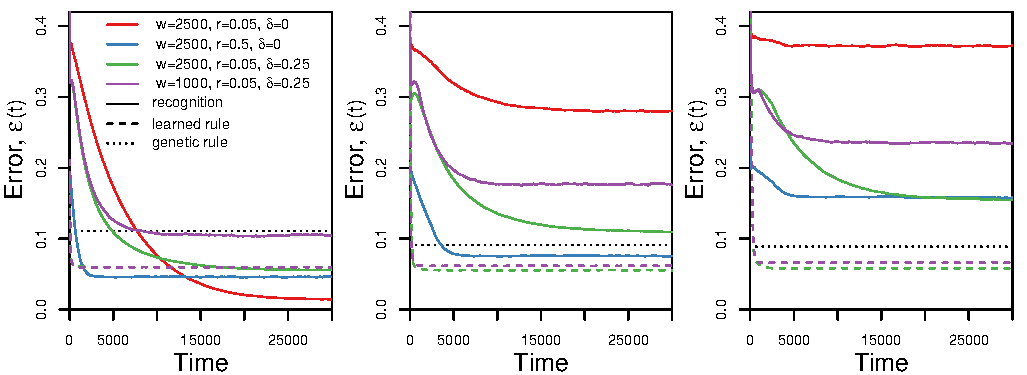
\includegraphics[width=.95\textwidth]{figures/learning_curves.pdf}
\caption{\label{learning_curves} \sffamily\small\textbf{Examples of how average error decreases over time.}
In each panel, we show time (in number of interactions) on the x-axis and learning error on the y-axis. The average error of each animal $i$ in each of the $25$ groups we model is $\epsilon_i$. The line shows the average of $\epsilon_i$ across all animals in all groups ($\bar{\epsilon}$), and the shaded area shows this average $\pm 0.5$ the standard deviation of $\epsilon_i$ across all animals in all groups. In each panel, blue lines show animals using individual recognition and red lines show animals using the badge system. The solid lines correspond to groups where signal-quality correlation is high ($\rho=0.9$) and the dotted lines correspond to groups where signal-quality correlation is lower ($\rho=0.5$). As memory window increases, from A to B, the error of animals using the badge system is not strongly affected, whereas the error of animals using individual recognition becomes lower. When group size becomes smaller, from B to C, the error of animals using both systems decreases, but it affects the error of animals using individual recognition more.  Parameters: in all panels $\delta = 0.5$, $p_\text{o}=0$; in A $N=50$, $w=300$; in B $N=50$, $w=1800$; in C $N=20$, $w=1800$. }
\end{figure}

\begin{figure}
%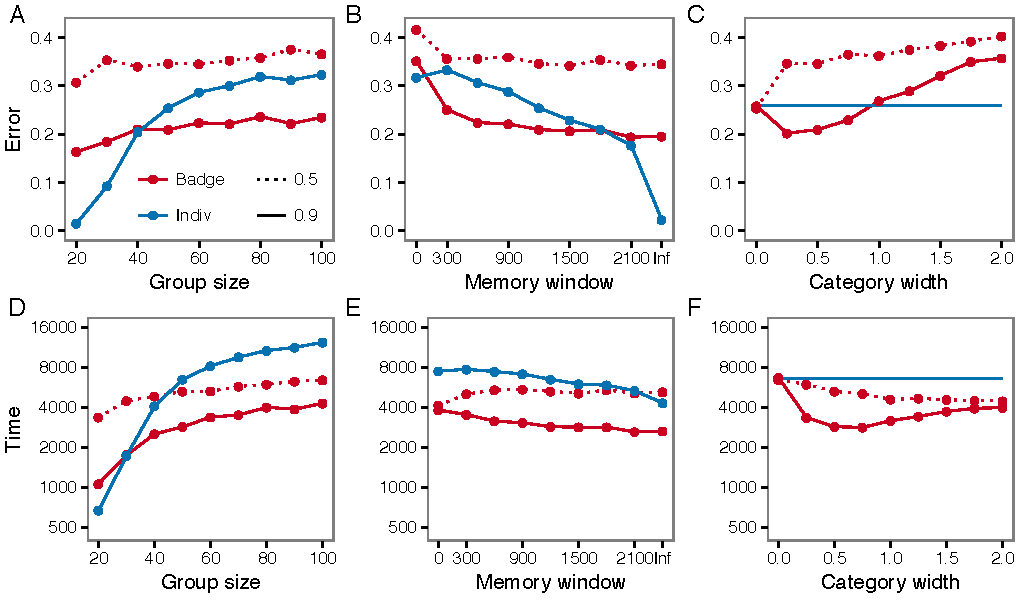
\includegraphics[width=6.85in]{figures/parameters.pdf}
\caption{\sffamily\small\textbf{Decreasing group size and increasing memory window both improve learning.} Error and learning time are minimized at an intermediate category width. Here we show average error ($\bar{\epsilon}$) (A-C) and average learning time ($\bar{\tau}$) (D-F) as a function of group size ($N$), memory window ($w$), and category width ($\delta$). In each panel, blue lines show animals using individual recognition and red lines show animals using the badge system. The solid red lines correspond to groups in which the signal-quality correlation $\rho=0.9$ and the dotted lines correspond to groups in which the signal-quality correlation $\rho=0.5$. Note that in this figure the animals do not use observational learning. Parameters: unless the parameter is being varied $\delta = 0.5$, $N=50$, $p_\text{o}=0$, $w=1200$.}
\label{parameters}
\end{figure}

\begin{figure}
%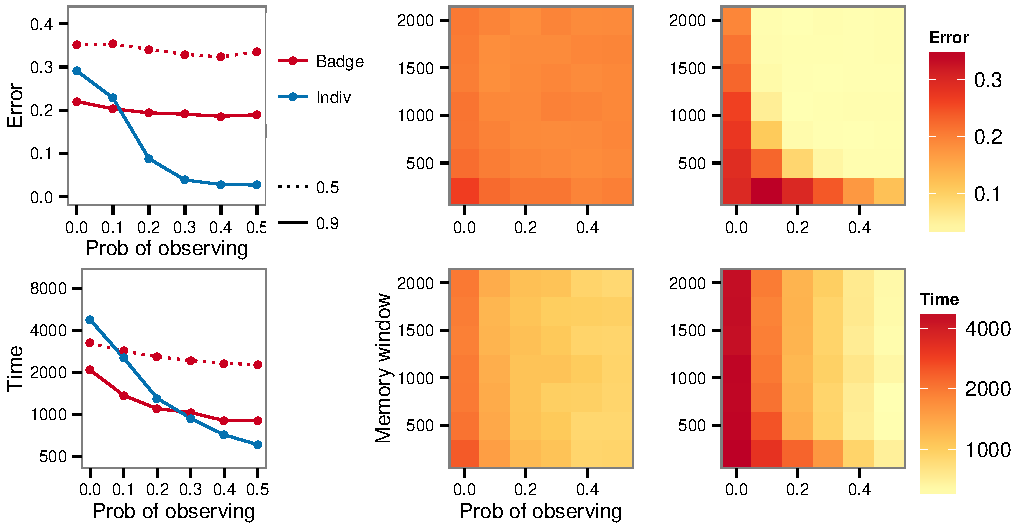
\includegraphics[width=6.85in]{figures/observational_learning.pdf}
\caption{\sffamily\small\textbf{Observational learning improves both error and learning time and does so much more for animals using individual recognition.} For animals using individual recognition, there is a strong interaction between the probability of observing and memory window. In A and D, we show average error ($\bar{\epsilon}$) and average learning time ($\bar{\tau}$), respectively, as a function of the probability of observing ($p_\text{o}$). In each panel, blue lines show animals using individual recognition and red lines show animals using the badge system. The solid red lines correspond to groups in which the signal-quality correlation $\rho=0.9$ and the dotted lines correspond to groups in which the signal-quality correlation $\rho=0.5$. In B and C we show average error ($\bar{\epsilon}$) as a function of both the probability of observing ($p_\text{o}$) on the horizontal axis and memory window ($w$) on the vertical axis. In E and F we show average learning time ($\bar{\tau}$) as a function of both the same parameters. The middle column shows these measures for animals using the badge system and the right column shows these measures for animals using individual recognition. Parameters: in all panels $\delta = 0.5$, $N=50$, $\rho=0.9$; in A and D $w=1200$, in B and E $\rho=0.9$.}
\label{observational}
\end{figure}

\begin{figure}
%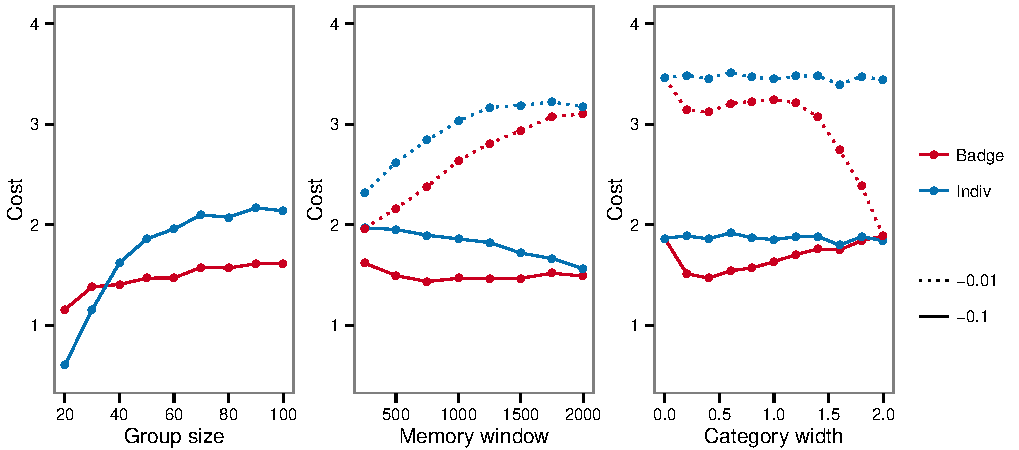
\includegraphics[width=6.85in]{figures/costs.pdf}
\caption{\sffamily\small\textbf{Overall costs are lowest in small groups.} When costs increase at low cognitive traits ($\alpha<1$), any increase in cognitive traits leads to an increase in overall cost, i.e. costs are lowest at low memory window and high category width. When costs increase at high cognitive traits ($\alpha>1$), intermediate cognitive traits are the least costly.  With individual recognition, costs decrease as the probability of observing increases. In each panel, we show overall costs ($C$) as a function of a particular parameter. Blue lines show animals using individual recognition and red lines show animals using the badge system. The solid lines correspond to $\alpha=5$ and the dotted lines correspond to $\alpha=0.2$.  Parameters: unless the parameter is being varied $\delta = 0.5$, $N=50$, $p_\text{o}=0$, $\rho=0.9$, $w=1200$.}
\label{costs}
\end{figure}
%LIZ comment: specify if this is with/without observational learning

\begin{figure}
%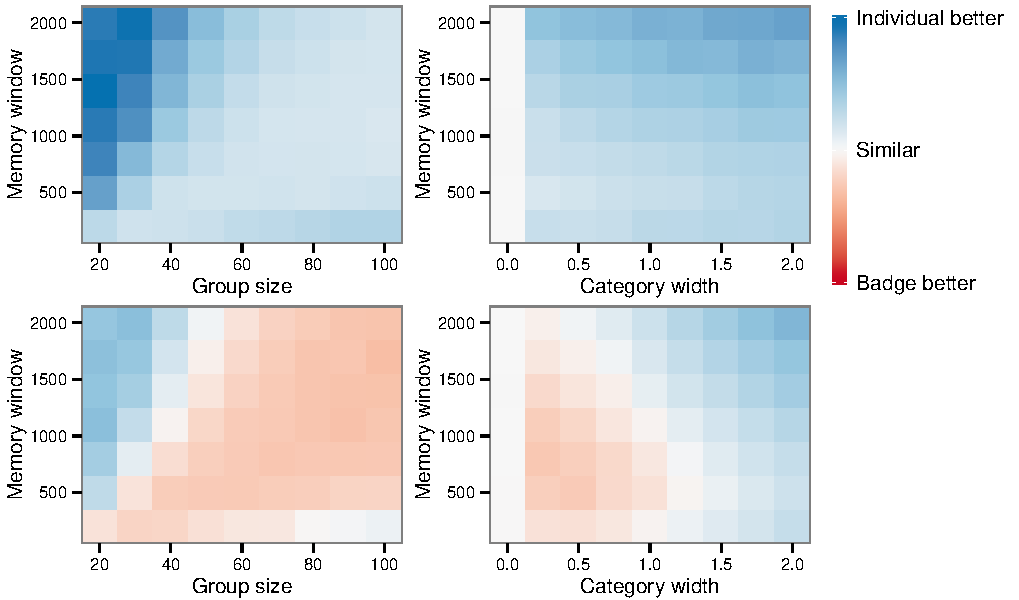
\includegraphics[width=6.85in]{figures/cost_comparisons.pdf}
\caption{\sffamily\small\textbf{The overall costs of using the badge system are lower than the costs of using individual recognition at high group size, low memory window, high category width, and small probability of observing.} When the signal-quality correlation $\rho$ increases, animals using the badge system incur lower costs for more combinations or parameters. Here we show the difference in the overall costs ($C$) associated with the badge system and with individual recognition as a function of pairs of two parameters. Red indicates the difference is negative, i.e. individual recognition is more costly, and blue indicates the difference is positive, i.e. individual recognition is less costly.  In the left column (A-D), the signal-quality correlation $\rho=0.9$, and in the right column (E-H), the signal-quality correlation $\rho=0.5$. Parameters: unless the parameter is being varied $\delta = 0.5$, $N=50$, $p_\text{o}=0$, $w=1200$.}
\label{comparison}
\end{figure}
%LIZ comment: specify if this is with/without observational learning

%
\begin {table}[ht]
\caption {Description of variables} \label{tab:vars} 
\begin{tabular}{cl}

 Variables & Description of variables \\
\midrule 
$C$ & total cost of learning \\ 
$c_\delta$ & inherent cost of using category width $\delta$ \\ 
$c_w$ & inherent cost of using memory window $w$ \\
$\delta$ & category width \\
$\epsilon_i$ & average error of animal $i$ about all other animals \\
$\bar{\epsilon}$ & average error of all animals in all groups \\
$\ell_\text{i}$ & learning rate in direct interaction, set to $0.2$ \\
$\ell_\text{o}$ & learning rate in indirect observation, set to $0.1$ \\
$N$ & number of animals in group \\ 
$p_\text{o}$ & probability of observing interactions between other pairs \\
 $q_i$ & quality of animal $i$ \\ 
 $\rho$ & correlation between quality and signal \\
$s_i$ & signal of quality / badge of status of animal $i$ \\ 
$\sigma_\text{b}$ & standard deviation of baseline opinion, set to $0.2$ \\
$\sigma_\text{i}$ & standard deviation of noise in opinion updating during interaction, set to $0.01$ \\
$\sigma_\text{o}$ & standard deviation of noise in opinion updating during observation, set to $0.02$ \\
$\sigma_\text{q}$ & standard deviation of quality values, set to $0.5$ \\
$T$ & total number of interactions, set to $20,000$ \\
$\tau_i$ & average learning time of animal $i$ \\
$\bar{\tau}$ & average learning time of all animals in all groups \\ 
$w$ & memory window 
\end{tabular}
\end {table}
% LIZ comment: add alpha parameter (shape/concavity of cost function?)

\setcounter{figure}{0}
\begin{figure}
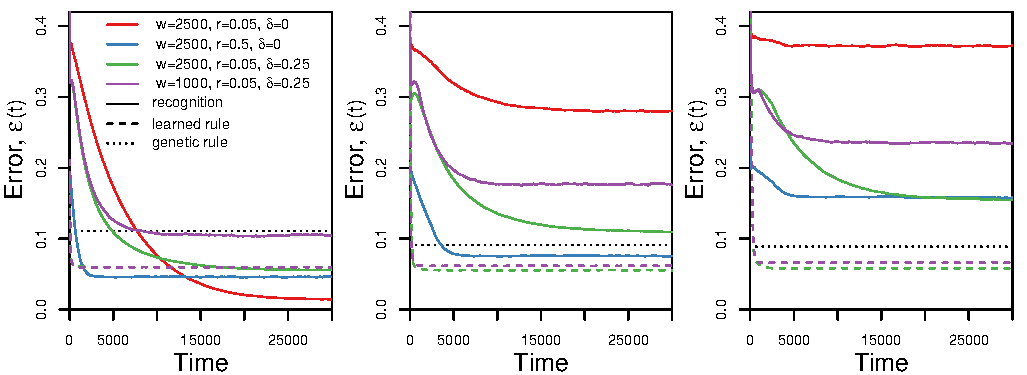
\includegraphics[width=.95\textwidth]{figures/learning_curves.pdf}
\caption{}
\end{figure}


\begin{figure}
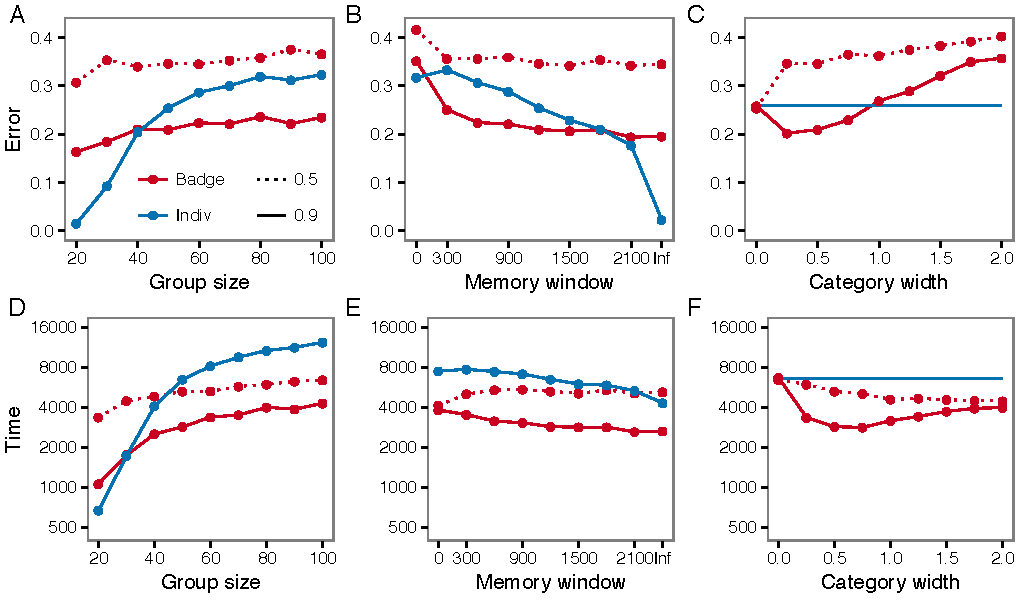
\includegraphics[width=6.85in]{figures/parameters.pdf}
\caption{}
\end{figure}

\begin{figure}
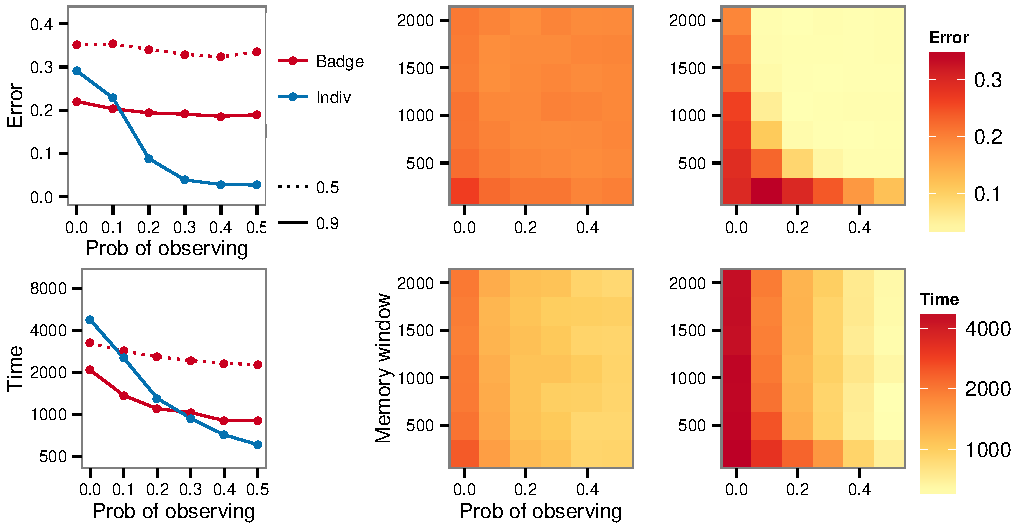
\includegraphics[width=6.85in]{figures/observational_learning.pdf}
\caption{}
\end{figure}

\begin{figure}
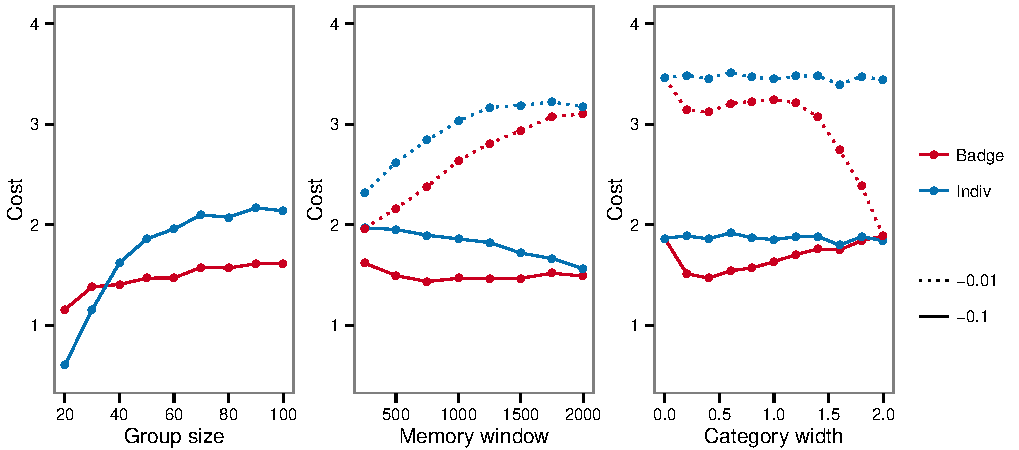
\includegraphics[width=6.85in]{figures/costs.pdf}
\caption{}
\end{figure}

\begin{figure}
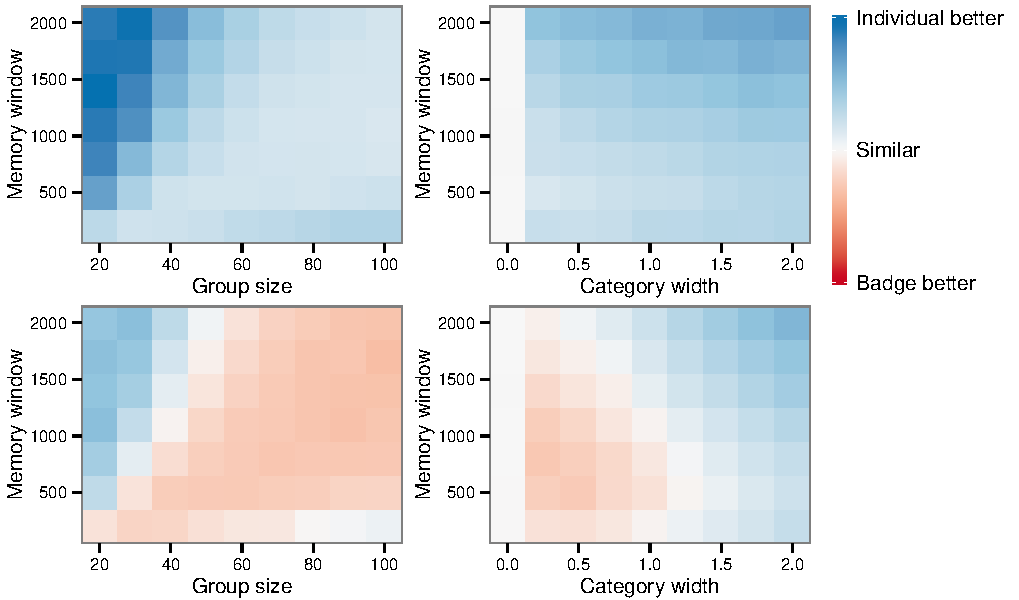
\includegraphics[width=6.85in]{figures/cost_comparisons.pdf}
\caption{}
\end{figure}

\clearpage{}
%\newpage{}
\renewcommand{\thesection}{}
\section{Supporting information}
\renewcommand{\thesection}{S}
\renewcommand{\thesubsection}{S\arabic{subsection}}
\renewcommand{\theequation}{S\arabic{equation}}
\renewcommand{\thetable}{S\arabic{table}}
\renewcommand{\thefigure}{S\arabic{figure}}
\setcounter{equation}{0}  
\setcounter{figure}{0}
\setcounter{table}{0}

\begin{figure}[ht]
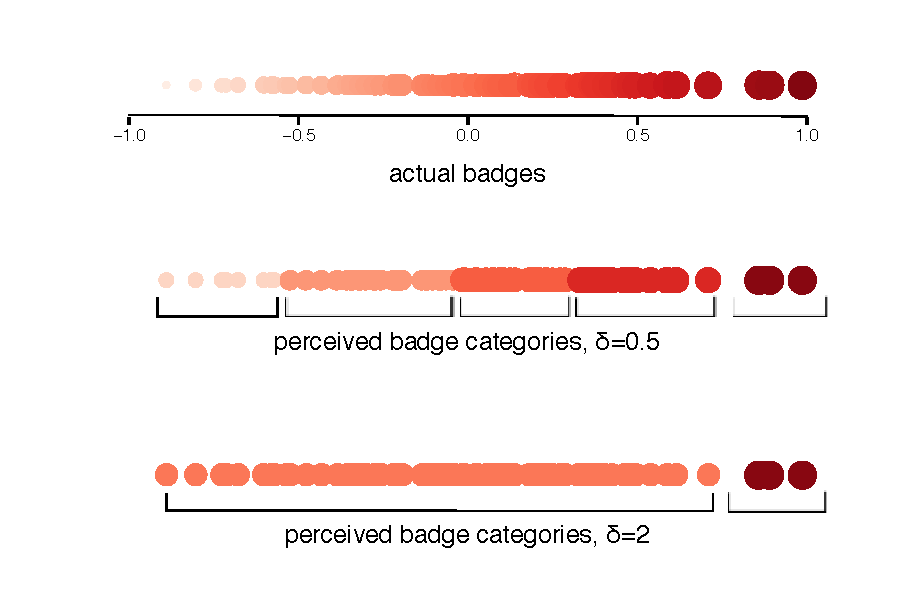
\includegraphics[width=.8\textwidth]{figures/categories.pdf}
\caption{\sffamily\small\textbf{Here we show an example of how a group of $N=100$ animals being divided into categories.} 
Each circle corresponds to an animal in the group. In each row, the horizontal position of the circle corresponds to its badge size. In the top row, the color and size of each circle indicate the size of each animal's badge. In the second and third rows, the color and size indicate the mean size of the badges of animals in each category, where categories were constructed using category width $\delta=0.5$ and $\delta=2$ respectively. Categories were formed by choosing an animal $i$ at random, putting all other animals whose signals were within $\delta/2$ of $i$'s signal $s_i$ into the same category, then choosing another uncategorized animal at random, and continuing until all animals were categorized.}
 \label{cats_ex}
\end{figure}

\begin{figure}[ht]
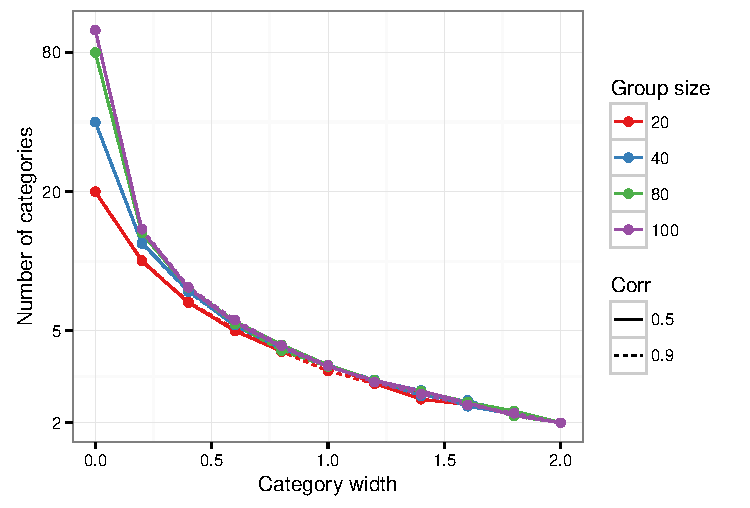
\includegraphics[width=.8\textwidth]{figures/number_of_categories.pdf}
\caption{\sffamily\small\textbf{As category width $\delta$ decreases the number of categories into which the group is divided increases.}
For a given group size $N$ and category width $\delta$ we generated a group with $N$ signal values $\{s_i\}$ and categorized the group according to the procedure in the text and Figure \ref{cats_ex} $100$ times and took the average number of categories across these $100$ iterations. Here we show how the average number of categories into which a group is divided depends on group size $N$ and category width $\delta$.  Each colored line corresponds to a group size. There are overlapping solid and dotted lines in each color since the signal-quality correlation $\rho$ does not affect the number of categories formed. When $\delta=0$ there are as many categories as there are animals in the group. When $\delta=2$, it is possible for all animals to be put into the same category, but in all $100$ iterations we simulated for each group size, there were $2$ categories. }
\label{num_cat}
\end{figure}

\begin{figure}[ht]
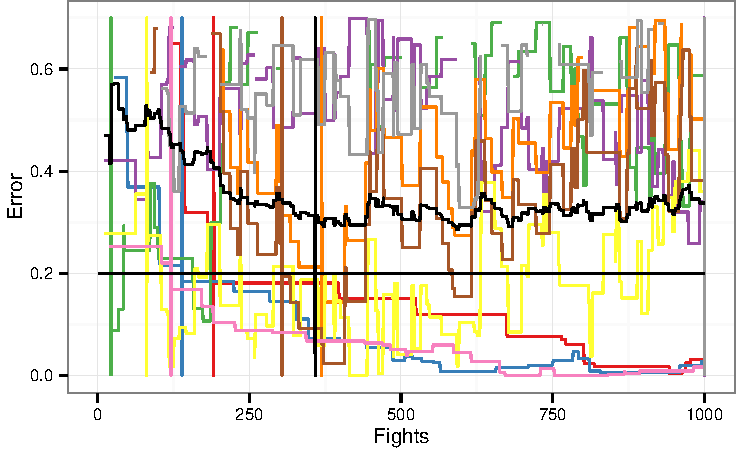
\includegraphics[width=.8\textwidth]{figures/learning_time_example.pdf}
\caption{\label{learnT.ex} \sffamily\small\textbf{Example of how to calculate learning time.} Learning time, $\tau_i$, can be less than $T$, even if average error at time $T$ is above the threshold $0.2$. Each colored line shows how one the error in one animal's opinion of its five group mates changes over time. The black line is its average error about the other animals ($\epsilon_i(t)$). The horizontal black line is the error threshold, $0.2$. Each vertical colored line is the first time when corresponding line drops below the threshold. The vertical black line is the average of these learning times  ($\tau_i$).}
\end{figure}

\begin{figure}[ht]
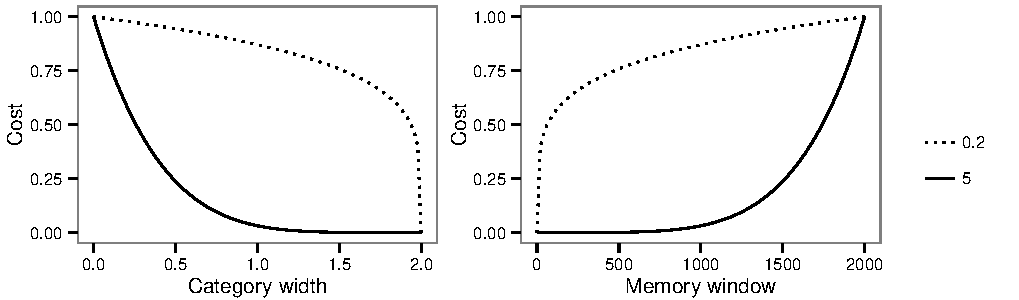
\includegraphics[width=.8\textwidth]{figures/cost_functions.pdf}
\caption{\sffamily\small\textbf{Cost functions.} Here we show how the cost functions for the cognitive parameters, category width $\delta$ and memory window $w$. In each panel, the solid line corresponds to $\alpha=5$ and the dotted line corresponds to $\alpha=0.2$. }
\label{cost_fx}
\end{figure}

%\begin{figure}[ht]
%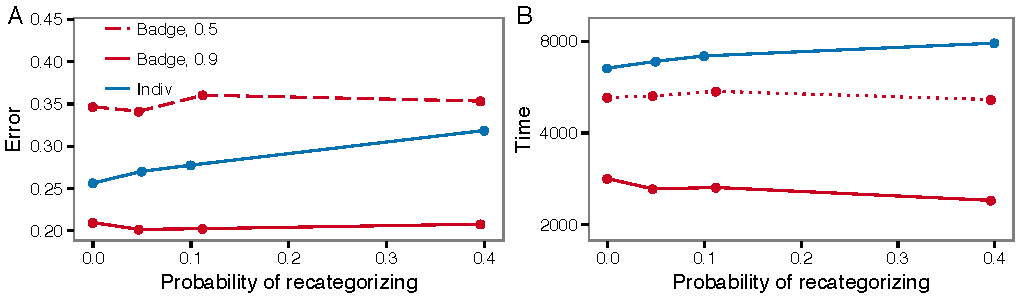
\includegraphics[width=6.85in]{figures/confusion_probs.pdf}
%\caption{\sffamily\small\textbf{Increasing the probability of being confused increases error and learning time in the individual recognition system and decreases error and learning time in the badge system.} Error and learning time are minimized at an intermediate category width. In the left panel, we show average error $\bar{\epsilon}$ as a function of the probability of recategorizing, and in the right panel, we show average learning time $\bar{\tau}$ as a function of the probability of recategorizing. In each panel, blue lines show animals using individual recognition and red lines show animals using the badge system. The solid red lines correspond to groups in which the signal-quality correlation $\rho=0.9$ and the dotted lines correspond to groups in which the signal-quality correlation $\rho=0.5$. Parameters: $\delta = 0.5$, $N=50$, $p_\text{o}=0$, $w=1200$.}
%\label{confusion_probs}
%\end{figure}

\begin{figure}[ht]
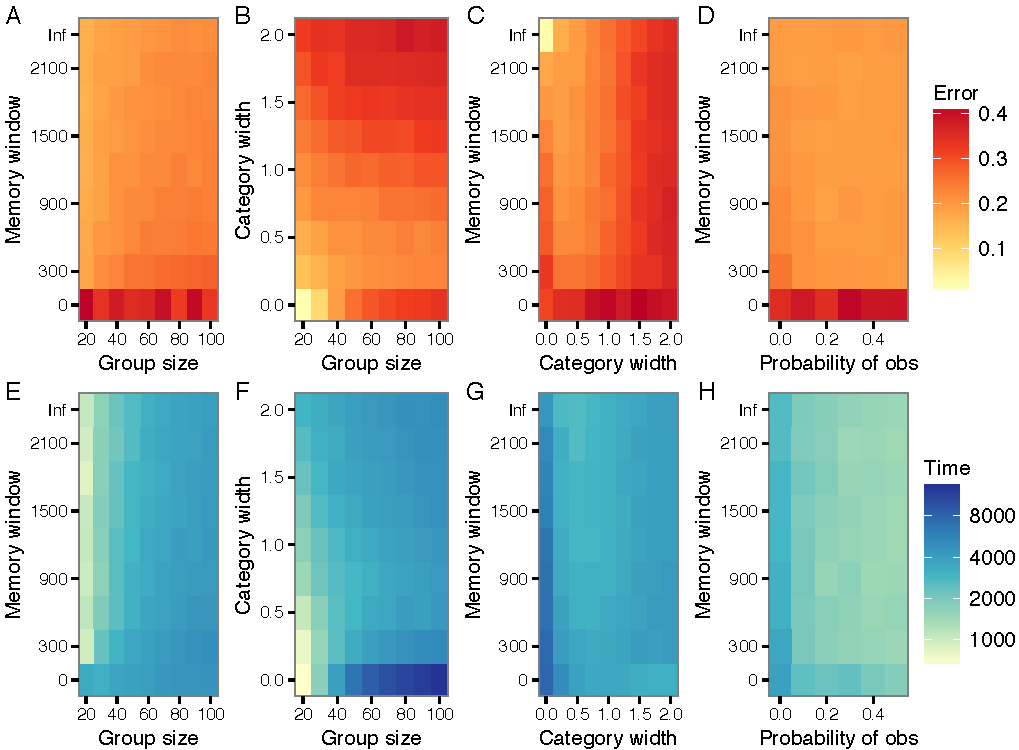
\includegraphics[width=.8\textwidth]{figures/parameter_interactions_badge.pdf}
\caption{\sffamily\small\textbf{Parameter interactions for animals using the badge system.}
In A-D we show average error ($\bar{\epsilon}$) for animals using the badge system as a function of two parameters. In E-H we show average learning time ($\bar{\tau}$) as a function of two parameters. Parameters: unless the parameter is being varied $\delta = 0.5$, $N=50$, $p_\text{o}=0$, $\rho=0.9$, $w=1200$.}
\label{interactions_badge}
\end{figure}

\begin{figure}[ht]
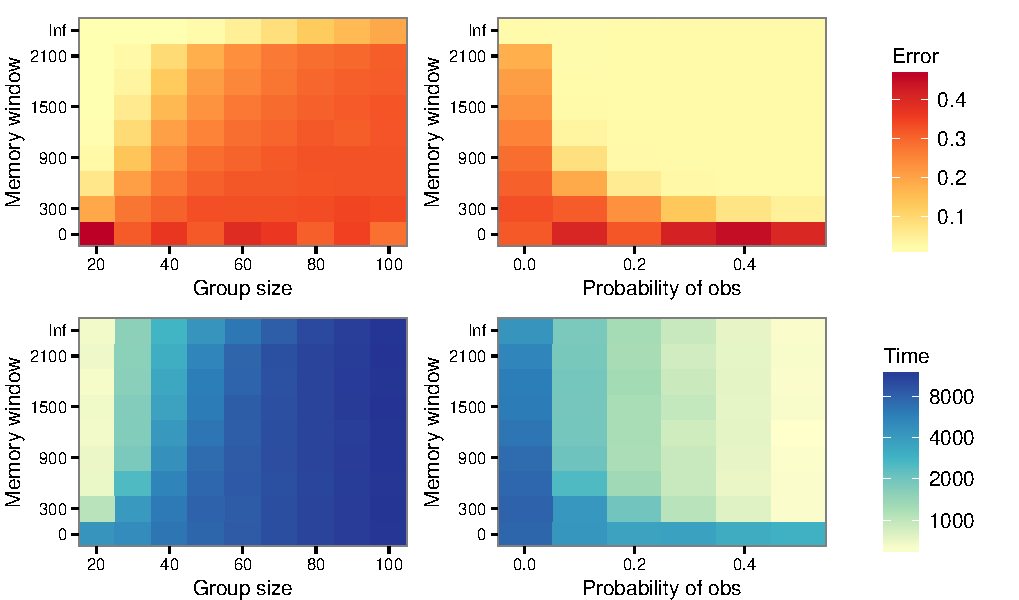
\includegraphics[width=.8\textwidth]{figures/parameter_interactions_indiv.pdf}
\caption{\sffamily\small\textbf{Parameter interactions for animals using individual recognition.}
In A and B we show average error ($\bar{\epsilon}$) for animals using individual recognition as a function of two parameters. In C and D we show average learning time ($\bar{\tau}$) as a function of two parameters. Parameters: unless the parameter is being varied $N=50$, $p_\text{o}=0$, $\rho=0.9$, $w=1200$.}
\label{interactions_indiv}
\end{figure}

\begin{table}
\caption{\label{corr_examples} Examples of the correlation between a badge and a measure of fitness.}
\begin{tabular}{lllll}
Species & Badge & Measure of fitness & Correlation & Reference
\\\hline paper wasp & percent black on face & head width & $r^2=0.36$, for wasps  & Tibbetts \& Dale 2004
\\ & & & with $\geq 2$ black spots
\\ & ``badge brokenness" & dominance & $r^2=.105$ & Tibbetts \& Dale 2004
\\ \hline house sparrow & size of black bib & physical condition & $r=0.379$ & Veiga 1993
\\ \hline swamp sparrow & size of rusty cap & parental investment & $r^2=0.33$ & Olsen et al. 2010
\\ & size of black forehead & aggression & $r^2=0.41$ & Olsen et al. 2010
\end{tabular}
\end{table}

\end{document}
